\section{Verteilungssicht}

In Abbildung~\ref{fig:deployment-diagram} ist eine Übersicht über das Deployment der Applikation und dazugehöriger
Services zu sehen.
\begin{figure}
    \centering
    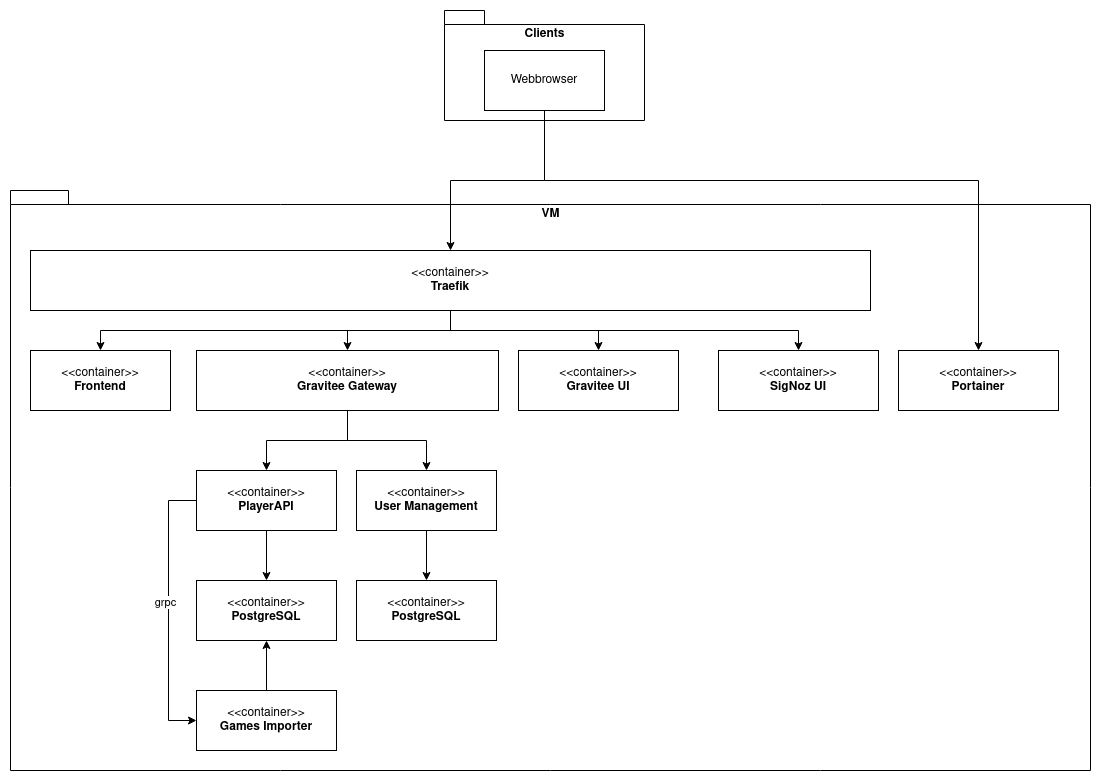
\includegraphics[width=\textwidth]{images/cdc-08-deployment-diagram.drawio}
    \caption{Deployment Diagramm}
    \label{fig:deployment-diagram}
\end{figure}

Die gesamte Applikation läuft innerhalb einer VM, wobei alles verdockert ist.
Das initiale Routing und bereitstellen von https Zertifikaten übernimmt Traefik (Edge Router).
So gibt es für jeden Teil eine eigene URL:
\begin{itemize}
    \item Frontend: lol-stats.de
    \item API (Gravitee Gateway): lol-stats.de/api
    \item Gravitee UI: api-ui.lol-stats.de
    \item SigNoz UI: tracing.lol-stats.de
    \item Grafana: grafana.lol-stats.de
\end{itemize}

Nur Portainer (Webseite zum Verwalten von Docker Stacks) ist direkt über einen Port erreichbar, weil es keine gute Idee ist Traefik in Portainer einzurichten
und gleichzeitig Portainer nur über Traefik erreichbar zu machen.
Alle API Anfragen werden über das Gravitee Gateway geleitet.
Gravitee ist eine API Management Software über die, die internen API Routen festgelegt werden.
Gravitee lässt sich über ein Webinterface in der Gravitee UI konfigurieren.
Die eingesammelten Traces lassen sich über ein Webinterface in der SigNoz UI anschauen.
Über Grafana (Datenvisualisierungstool) lassen sich die von Loki (Log-Aggregierung-Tool) eingesammelten Logs durchsuchen.
